\documentclass[a4paper,10pt]{scrartcl}
\usepackage[utf8]{inputenc}
\usepackage[T1]{fontenc}
\usepackage{booktabs}
\usepackage{import}
\usepackage{xspace}
\usepackage{enumitem}
\usepackage{cite}
\usepackage{graphicx}
\usepackage{tikz}
\usepackage{wrapfig}
\usepackage{pdflscape}
\usetikzlibrary{arrows}
\usetikzlibrary{fit}
\usetikzlibrary{calc}
\usepackage{float}
\usepackage{amssymb}
\usepackage{listings}
\usepackage[section]{placeins} % don't move figures beyond the next section heading

% this is needed for forms and links within the text
\usepackage{hyperref}

% Variables
\newcommand{\authorName}{
   Mohammed~Abu~Jayyab,
   Niklas~Baumstark,
   Tobias~Gräf,
   Amrei~Loose,
   Christoph~Michel
}
\newcommand{\authorNameEmph}{
   Mohammed~Abu~Jayyab,
   \textbf{Niklas~Baumstark},
   Tobias~Gräf,
   Amrei~Loose,
   Christoph~Michel
}

\newcommand{\dateFirstVersion}{\today}
\newcommand{\customer}{Karlsruhe Institute of Technology}
\newcommand{\contractor}{A company}
\newcommand{\projectName}{Broadcast Encryption\xspace}

\newcommand{\doctitle}{\projectName (Implementation)}
\title{\doctitle}
\author{\authorName}
\date{\today}

% less margin
\usepackage[margin=2.5cm]{geometry}

% horizontal line
\newcommand{\HRule}{\rule{\linewidth}{0.5mm}}

% more beautiful lists
\setlist{noitemsep}
\renewcommand{\labelitemi}{$\bullet$}
\renewcommand{\labelitemii}{$\diamond$}

% create a shorter version for tables
\newcommand\addrow[2]{#1 &#2\\ }
\newcommand\addheading[2]{\textbf{\sffamily #1} &\textbf{\sffamily #2}\\ \hline}
\newcommand\tabularhead{\begin{tabular}{lp{13cm}}
\hline
}

\newcommand\addmulrow[2]{ \begin{minipage}[t][][t]{2.5cm}#1\end{minipage}%
   &\begin{minipage}[t][][t]{8cm}
    \begin{enumerate} #2   \end{enumerate}
    \end{minipage}\\ }

\newenvironment{usecase}{\tabularhead}
{\hline\end{tabular}}

% a cross
\newcommand\X{$\times$}

% templates and default styles for figures and graphics
\tikzset{>=triangle 45}
\tikzset{font=\sffamily}

\newcommand{\tmpCaption}{}
\newenvironment{illustration}[1]
{
   \renewcommand{\tmpCaption}{#1}
   \begin{figure}[h!]
   \centering
}
{
   \caption{\tmpCaption}
   \end{figure}
}


\begin{document}

\maketitle
  \begin{tabular}[t]{ll}
	Projekt:       & \quad \projektName \\[1.2ex]
	Auftraggeber:  & \quad \auftraggeber\\[1.2ex]
	Auftragnehmer: & \quad \auftragnehmer\\[1.2ex]
  \end{tabular}

\begin{tabular}{|p{3 cm}|p{3 cm}|p{5 cm}|}
\hline
\textbf{Version} & \textbf{Datum} & \textbf{Autor(en)} \\
\hline
\hline
1.0 & 29.04.2012 & \authorName \\
\hline
\end{tabular}

\tableofcontents
\clearpage

\section{Introduction}
This document aims to describes the rationale behind changes that were applied to the initial design
in the course of implementing the CryptoCast project. One can find the final, complete API specification (including new UML-diagrams)
in an updated version of the design document.

\section{General changes}
\begin{itemize}
   \item In addition to the Java implementation some of the methods were implemented in C++ in order to increase the perfomance
	of mathematical operation used by the cryptography.
   \item Maven 3 was introduced as a build-system.
   \item As described in 3.6 cryptocast.client the minimal API level of the client has changed from 8 to 10.
\end{itemize}

\section{API Changes}
The following sections contain the classes and their changes ordered by packages. As in the introduction already mentioned, every
changed class is annotated with further details.
\subsection{\lstinline|cryptocast.comm|}

\begin{itemize}

  \item \lstinline|SimpleHttpStreamServer|
  \begin{itemize}
   \item This class was added to have a working HTTP implementation to supply Android's
    \lstinline|MediaPlayer|.
  \end{itemize}

   \item \lstinline|MessageBuffer|
  \begin{itemize}
   \item Added solely for testing purposes.
  \end{itemize}

   \item \lstinline|StreamUtils|
  \begin{itemize}
   \item Added several utility function for the implementation of the \lstinline|cryptocast.comm| package.
  \end{itemize}

   \item \lstinline|ThrottledOutputStream|
  \begin{itemize}
   \item Added because we needed a way to throttle a media stream to the bitrate of the source file.
  \end{itemize}

  \item \lstinline|SwitchableOutputStream|
  \begin{itemize}
   \item Added for usage in the server controller when doing a reinitialization.
  \end{itemize}

  \item \lstinline|SwitchableInputStream|
  \begin{itemize}
   \item Added for on-the-fly switching of the media source in the server controller.
  \end{itemize}

  \item \lstinline|MessageInChannel|, \lstinline|MessageOutChannel|
  \begin{itemize}
   \item Transformed into an interface, because there is more than one sensible implementation.
   \lstinline|StreamMessage{In,Out}Channel| realize the reference implementation based on streams.
  \end{itemize}

  \item \lstinline|MultiOutChannel|
  \begin{itemize}
   \item Replaces the \lstinline|MultiOutStream|. We realized that we need multiplexing on a
         message level, rather than on the stream level, so we don't need message synchronization
         on the receiver end.
  \end{itemize}

  \item \lstinline|ServerMultiMessageOutChannel|
  \begin{itemize}
   \item Replaces \lstinline|ServerMultiMessageOutChannel| because we need multiplexing
   on a message level (see above).
   \item Added the possibility to register an error handler.
  \end{itemize}
\end{itemize}

\subsection{\lstinline|cryptocast.server|}

\begin{itemize}

\item \lstinline|Controller|
\begin{itemize}
 \item Added backend functions for the newly designed shell commands.
 \item Added convenience methods for usage in the shell.
\end{itemize}

\item \lstinline|ServerData<ID|
\begin{itemize}
  \item Transformed into an abstract class. All the functionality in here is now
        independent of the NP scheme. The reference implementation that is used for
        NP is called \lstinline|NaorPinkasServerData|.
  \item Added an interface to revoke multiple users (because revoking users must cause a
        key update!)
\end{itemize}

\item \lstinline|LogbackUtils|
  \begin{itemize}
   \item Convenience functions to configure Logback's output.
  \end{itemize}

\item \lstinline|OptParse|
\begin{itemize}
  \item Convenience when working with command line arguments and the \emph{JCommander} library.
\end{itemize}

\end{itemize}

\subsection{\lstinline|cryptocast.server.programs|}
All the main programs are added here. Most notably, theses are:
\begin{itemize}
 \item \lstinline|Benchmarks| Several benchmarks for various operations that the
   server and client need to perform.
 \item \lstinline|Server|  The CryptoCast server.
\end{itemize}

\subsection{\lstinline|cryptocast.client|}

Due to missing functionality in Android's \lstinline|MediaPlayer| class (for example: buffer callback was not triggered), we decided to upgrade the minimal API level to 10. This decision was made to ensure better feedback for the user about the current status of the program. So for example, the user can see whether the client is currently buffering or not and can react accordingly.

\begin{itemize}
\item \lstinline|StreamViewerActivity| \newline
   This class now implements  \lstinline|MediaController.MediaPlayerControl| to provide better
  control of the media player. In addition, the following methods were added:
  \begin{itemize}
   \item \lstinline|+setStatusText(...)| to set the player's status text.
   \item \lstinline|+createErrorPopup(...)| to create an error popup from other classes.
  \end{itemize}

   \item \lstinline|MainActivity|
  \begin{itemize}
   \item \lstinline|+connectToServer(...)| was renamed to \lstinline|+onConnect(...)|.
   \item \lstinline|+onOldServers(...)| was added to start a new server fragment for showing the
    list of all servers.
    \item \lstinline|+getConnectAddr()| was added to get the socket address
    and to check, if the host name and the port number are valid.
  \end{itemize}

  \item \lstinline|ServerHistory| \newline
  The following methods were added :
  \begin{itemize}
   \item \lstinline|+deleteServer(...)| to delete a server from the server history.
   \item \lstinline|+invalidateKeyFile(...)| to delete a saved key file of the server.
   \item \lstinline|+getKeyFile(...)| to return the key file of the given server.
   \item \lstinline|+getServerList()| to return a list of the saved servers, that simplifies the access for listing them in options and main menu.
  \end{itemize}

 \item \lstinline|ClientActivity|
  \begin{itemize}
   \item This class was added as base activity, which provides basic common functionality like the menu.
  \end{itemize}

    \item \lstinline|ClientApplication|
  \begin{itemize}
   \item This class was added for maintaining the global application state.
  \end{itemize}

  \item \lstinline|HelpActivity|
  \begin{itemize}
   \item This class was added to represent an activity that displays the help page.
  \end{itemize}

  \item \lstinline|AboutActivity|
  \begin{itemize}
   \item This class was added to represent the about dialog.
  \end{itemize}

   \item \lstinline|MessageFragment|
  \begin{itemize}
   \item The class \textit{"ErrorFragment"} was renamed to \textit{"MessageFragment"}.
  \end{itemize}

  \item \lstinline|ServersFragment|
  \begin{itemize}
   \item This class was added to represent a dialog with a list of all saved servers and a button.
  \end{itemize}

  \item \lstinline|ServerListAdapter|
  \begin{itemize}
  \item This class was added to provide an adapter between the ListElements and the view showing them. It extends an ArrayAdapter, but changes the way the InetSocketAddress is presented, by not using the toString() method.
  \end{itemize}

  \item \lstinline|RawStreamMediaPlayer|
  \begin{itemize}
  \item This class was added to provide Media player to play audio from a raw InputStream.
  \end{itemize}

  \item \lstinline|StreamConnector|
  \begin{itemize}
  \item This class was added to separate work from the StreamViewerActivity class
  in a separate thread to prevent the GUI not from showing properly.
  \end{itemize}

  \item \lstinline|OptionsActivity|
  \begin{itemize}
  \item \lstinline|+onCreateContextMenu(...)| was added to
  create a context menu to edit the server history.
  \item \lstinline|+onContextItemSelected(...)| was added to edit the selected item in the server history
    \end{itemize}

  \item \lstinline|KeyChoiceActivity|
  \begin{itemize}
  \item Methods were removed because the key file arguments are passed new via \lstinline|getIntent().getExtras()|.
  \end{itemize}



\end{itemize}


\subsection{\lstinline|cryptocast.client.filechooser|}

\begin{itemize}

 \item \lstinline|class NavigateUpListElement|
  \begin{itemize}
   \item This class was added as a list element in our file chooser representing a directory.
  \end{itemize}

    \item \lstinline|class FileChooserState|
  \begin{itemize}
   \item This class was added to represent the state of a file chooser.
  \end{itemize}

\end{itemize}

\subsection{\lstinline|cryptocast.util|}

Mostly everything in this package are helper functions that were extracted from code
in other packages during refactoring.

\begin{itemize}
  \item \lstinline|OptimisticGenerator|
  \begin{itemize}
   \item Provides a very generic and powerful abstraction of a range generator. We use this
   for the user key generation, because our polynomial evaluation algorithm is fast only
   if we generate keys in bulks. So we just compute the keys in blocks of powers of two.
   The result is that we never have more than $2n$ keys ready, where $n$ is the number of users
   and that we can dynamically grow the number of users efficiently.
  \end{itemize}

  \item \lstinline|CanBeObserved|
  \begin{itemize}
   \item This interface was added because we need it in the declaration of \lstinline|NPServerInterface|,
   where we can't use the abstract class \lstinline|java.util.Observable|
  \end{itemize}

  \end{itemize}

\subsection{\lstinline|cryptocast.crypto|}

\begin{itemize}
   \item \lstinline|BroadcastSchemeUserManager|
   \begin{itemize}
     \item Revocation of users is a costly operation: A new session key must be encrypted
     using Naor-Pinkas and decrypted on the client side. If a user wants to revoke multiple
     users, he needed to do so using repeated calls to the \lstinline|revoke| method.
     A straightforward implementation of \lstinline|BroadcastEncryptionServer| just triggers
     a key update whenever a user is revoked. Since this is the implementation we decided to
     stick with, we provide a method to revoke multiple users at once, triggering only
     a single key update. This method is exposed to the user by an extension of the \lstinline|revoke| command
     in the server shell.
  \end{itemize}

   \item \lstinline|CyclicGroupOfPrimeOrder|
  \begin{itemize}
    \item Captures the common interface between the DDH groups we support:
   \lstinline|SchnorrGroup| and \lstinline|EllipticCurveGroup|. A great advantage
   is that we can formulate multiexponentation using Shamir's trick generically. Even more importantly,
   we can formulate the Naor-Pinkas-Scheme completely independently from the group we use!
  \end{itemize}

   \item \lstinline|CryptoUtils|
  \begin{itemize}
   \item Simple helper methods for one-shot encryption and decryption using AES. We use this
   to encrypt the session key with the shared Naor-Pinkas secret. We also add a function that
   encrypts a hashed version of a plain text, so we notice when we obtain the wrong session
   key because we used a keyfile for the wrong server (because Lagrange interpolation will work,
   it will just give us a wrong result).
  \end{itemize}

  \item \lstinline|DynamicCipherInputStream|, \lstinline|DynamicCipherOutputStream|
  \begin{itemize}
   \item These classes provide the core abstraction of out broadcast scheme protocol: They
   implement the network protocol used between a server and the clients. \\
   It is based on symmetric encryption with a session key that can be changed at any
   time during transmission.
   The protocol works with two types of messages: Payload messages and key updates.
   Payload messages contain AES-encrypted data and key update messages contain a new session key,
   encrypted and decrypted with an abstract \lstinline|Encryptor|/\lstinline|Decryptor| pair. \\
   In the case of CryptoCast, the two instances use the Naor-Pinkas scheme to communicate
   the secret between the server and authorized clients.
  \end{itemize}

  \item \lstinline|EllipticCurve|, \lstinline|EllipticCurveOverFp|, \lstinline|EllipticCurveGroup|
  \begin{itemize}
   \item Provide the mathematical means to implement Naor-Pinkas based on elliptic curves.
   The common structure of \lstinline|EllipticCurveGroup| and \lstinline|SchnorrGroup| is
   captured by  \lstinline|CyclicGroupOfPrimeOrder| (see above).
  \end{itemize}

   \item \lstinline|DecryptionError|, \lstinline|InsufficientInformationError|, \lstinline|NoMoreRevocationsPossibleError|
  \begin{itemize}
   \item Exception classes for different parts of our algorithms.
  \end{itemize}

  \item \lstinline|SchnorrGroup|
  \begin{itemize}
   \item Represents the mathematical structure that is used in the Naor-Pinkas paper
   to implement the scheme.
  \end{itemize}

\end{itemize}

\subsection{\lstinline|cryptocast.crypto.naorpinkas|}

The prefix of the \lstinline|NaorPinkas{Name}| classes was changed to just \lstinline|NP{Name}| for readability.

Since we decided to provide an implementation of NP based on elliptic curves, we needed to extract
the common parts of the algorithm to avoid code duplication.

However, the server needs to work with both implementations, so a common facade is also needed.

Also, due to the different implementations, type arguments were introduced to tie an instance
to a specific underlying type of group. This introduces compiler-checked guarantees that prevent
confusion between the different implementations and avoids casting.

\begin{itemize}
  \item \lstinline|NPServerInterface|
  \begin{itemize}
    \item Describes the interface of the NP server that is available to users of the API.
          This is what the CryptoCast server uses.
  \end{itemize}

  \item \lstinline|NPServerFactory|
  \begin{itemize}
    \item Describes a strategy to generate server instance. Implementations are
          \lstinline|ECNPServerFactory| and \lstinline|SchnorrNPServerFactory|, which
          create the differrent server implementations.
  \end{itemize}
\end{itemize}

\section{Statistics}
To get a rough overview of compexity of the source code you can regard the following numbers.
The projects consists currently of:
\begin{itemize}
    \item  about 7400 lines of code, containing 1700 lines of tests and 400 lines of code written in C++.
    \item 140 Java-files.
    \item 189 types.
    \item an average of 6 lines of code per method, 2 fieldsper type and 2 methods per type (of course in a few cases differs a lot from this value).
\end{itemize}

\section{Approximate time plan}

The following diagram was created by examining the Git commit log of the project. It shows
the places of the code base we worked on at different stages of the implementation.
\newline
\begin{illustration}{An approximate time table of the project}
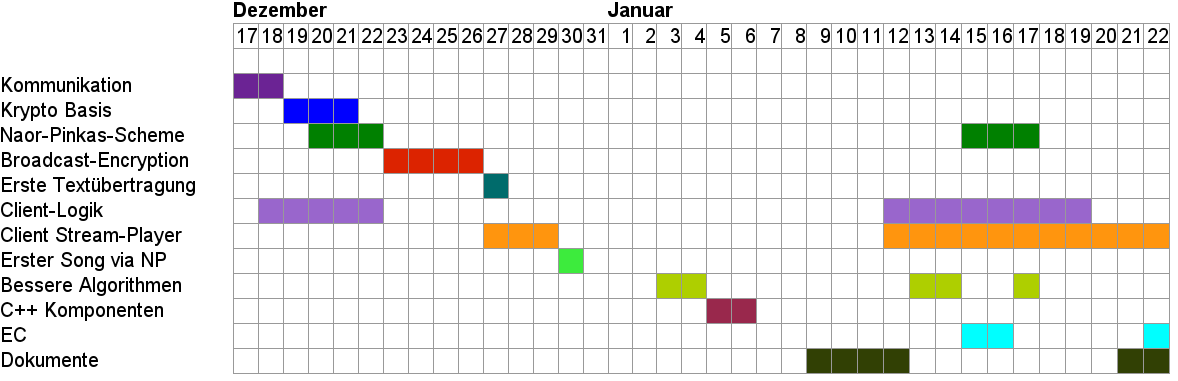
\includegraphics[width=400px]{timetable.png}
\end{illustration}

The chart shows that a lot of time was needed to implement the client UI. The main reason
for this is that we tried different approaches to work around the broken \lstinline|MediaPlayer|
implementation in Android API Level 8. We finally solved this by upgrading to API Level 10,
where the implementation is a lot more mature.

Towards the end of the implementation phase, we put most of the effort into creating a Naor-Pinkas
backend based on elliptic curve cryptography and adding performance optimizations.

\end{document}

